% ================================================================
% VALID: A 12-Item Validation Checklist for Financial ML
% KDD-MLF 2026 — ACM sigconf, 8p content, double-blind
% ================================================================
\documentclass[sigconf,anonymous,review]{acmart}

\usepackage{booktabs}
\usepackage{graphicx}
\usepackage{xcolor}
\usepackage{amsmath,amssymb}
\usepackage{multirow}
\usepackage{array}

% suppress ACM-specific fields for submission
\settopmatter{printacmref=false}
\renewcommand\footnotetextcopyrightpermission[1]{}
\pagestyle{plain}
\acmConference[KDD-MLF '26]{9th ACM SIGKDD Workshop on Machine Learning in Finance}{August 2026}{Jeju, Republic of Korea}
\acmYear{2026}

\begin{document}

\title{VALID: A 12-Item Validation Checklist for Financial Machine Learning}

\begin{abstract}
Machine learning strategies for cryptocurrency trading routinely
report exceptional backtest results, yet practitioners consistently
fail to replicate them. No domain-specific validation standard
exists for financial ML. We introduce VALID, a 12-item validation
checklist---the first domain-specific checklist addressing temporal
leakage, backtest overfitting, cost modeling, and class imbalance
in financial ML.

An audit of 80 published papers reveals the median study satisfies
only 2.5 of 12 items. Applying VALID to 340 strategy variants
across three assets and four timeframes, we document three failure
modes: directional prediction bias (90--97\%), statistical-economic
disconnect, and cost illusion (55--91\% alpha erosion). Monte Carlo
analysis ($n=200$) shows 27\% false positive rates under standard
validation, reduced to 0\% by CPCV with PBO. Even strategies
surviving multiple testing correction exhibit certain overfitting
under CPCV. We release an open-source implementation and discuss
implications for validating LLM-based trading systems.
\end{abstract}

\keywords{financial machine learning, validation framework, backtest
overfitting, cryptocurrency trading, reporting standard}

\maketitle

% ================================================================
\section{Introduction}
\label{sec:intro}
% ================================================================

Our audit of 80 published cryptocurrency ML papers reveals that the
median study satisfies only 2.5 of 12 basic validation items. The
consequences are predictable: strategies reporting exceptional in-sample
performance consistently fail out-of-sample, replicating the broader
pattern identified by~\citet{ioannidis2005false} in biomedical research
and by~\citet{harvey2016cross} in equity factor literature, where the
majority of 316 published factors are likely false
discoveries.~\citet{mclean2016academic} documented 58\% post-publication
decay in return predictability;~\citet{wiecki2016glitters} analyzed 888
algorithmic strategies and found near-zero correlation between backtest
and live Sharpe ratios.

Domain-specific reporting checklists have demonstrably improved research
quality in other fields. TRIPOD~\cite{collins2015tripod} (22~items,
10{,}000+ citations) transformed clinical prediction methodology.
REFORMS~\cite{kapoor2024reforms} addresses general ML science with 32
items. Yet \textbf{no published standard addresses financial ML}---a
domain with unique challenges including temporal data dependencies,
transaction cost modeling, structural class imbalance, and the
distinction between statistical and economic significance.

This paper makes three contributions:

\begin{enumerate}
\item \textbf{VALID}: a 12-item validation checklist for financial
ML---the first domain-specific framework for this field.

\item \textbf{Three failure modes at scale}: using 340 strategy variants
across three assets and four timeframes, we document directional
prediction bias, statistical-economic disconnect, and cost illusion.

\item \textbf{Monte Carlo FPR quantification}: AUC-based validation
produces 27\% false positives; CPCV with PBO reduces this to 0\%.
Multiple testing correction (Bonferroni) leaves nine ``significant''
strategies---all with PBO\,=\,1.0, proving that standard corrections
alone cannot detect backtest overfitting.
\end{enumerate}


% ================================================================
\section{Related Work}
\label{sec:related}
% ================================================================

\subsection{Backtest Overfitting and Validation Methodology}

The theoretical foundations for detecting backtest overfitting are
well established. The Reality Check of White~\cite{white2000reality}
and the Superior Predictive Ability test of
Hansen~\cite{hansen2005test}
address data snooping in multiple hypothesis testing.
Bailey et~al.~\cite{bailey2017pbo} introduced the Probability of
Backtest Overfitting (PBO) and the Deflated Sharpe Ratio (DSR),
providing the first formal tools for quantifying strategy selection
bias. Arian et~al.~\cite{arian2024backtest}, published in
\emph{Knowledge-Based Systems}, compared CPCV against walk-forward
methods in a synthetic controlled environment, confirming CPCV's
superior false-positive control.
Witzany~\cite{witzany2021bayesian} provided the only formal critique
of PBO, demonstrating that it exhibits negative bias when strategy
returns are similar---a finding we confirm empirically in
Section~\ref{sec:stat-econ}.

Empirically, Wiecki et~al.~\cite{wiecki2016glitters} analyzed 888
algorithmic trading strategies from the Quantopian platform and found
that backtest Sharpe ratio has near-zero predictive power for
out-of-sample performance ($R^2 < 0.025$). Our analysis of 340 ML
cryptocurrency strategies follows an analogous large-cohort evaluation
design.

\subsection{Reporting Standards for ML Research}

Domain-specific reporting checklists have demonstrated substantial
impact on research quality. In clinical prediction,
TRIPOD~\cite{collins2015tripod} (22~items) has accumulated over
10{,}000 citations and measurably improved methodological transparency.
Its ML extension, TRIPOD+AI~\cite{collins2024tripodai} (27~items),
and the LLM-specific TRIPOD-LLM~\cite{gallifant2025tripodllm}
(19~items, 50~subitems) further broaden coverage. In general ML
research, REFORMS~\cite{kapoor2024reforms} proposes 32~items, while
Model Cards~\cite{mitchell2019model} and Datasheets for
Datasets~\cite{gebru2021datasheets} address model and data
documentation respectively---each accumulating thousands of citations
without proposing novel algorithms.

Critically, \textbf{no published reporting standard addresses
financial ML}. Neither REFORMS nor TRIPOD+AI covers transaction cost
modeling, class imbalance in directional prediction, temporal
cross-validation with purge/embargo, or the distinction between
statistical and economic significance. VALID fills this gap.

\subsection{The ``Most Research Is Wrong'' Tradition in Finance}

VALID enters a well-established intellectual lineage.
Harvey et~al.~\cite{harvey2016cross} cataloged 316 published equity
factors and argued that most are likely false discoveries, requiring
$t$-statistics above 3.0. McLean and
Pontiff~\cite{mclean2016academic} documented 58\% post-publication
decay in return predictability. Novy-Marx and
Velikov~\cite{novymarx2016taxonomy} showed that most equity anomalies
with high turnover become unprofitable after costs---a finding we
extend to cryptocurrency ML in Section~\ref{sec:cost}.
More recently, Karl et~al.~\cite{karl2024embracing} formally argued
at ICML~2024 that negative results in ML prevent community-wide
resource waste, providing direct methodological support for VALID's
approach. Successful negative-result papers in adjacent domains---such
as Grinsztajn et~al.~\cite{grinsztajn2022tree} (trees outperform
deep learning on tabular data) and Zeng
et~al.~\cite{zeng2023transformers} (linear models outperform
Transformers for time series)---demonstrate that rigorous
disconfirmation, paired with constructive alternatives, consistently
achieves high impact.

In cryptocurrency specifically, the validation landscape remains
barren. Our audit of 80 papers (Section~\ref{sec:audit}) finds 0\%
CPCV adoption, 72\% class imbalance neglect, and 53\% cost omission.
VALID addresses this gap by synthesizing the theoretical tools of
Bailey and L\'{o}pez de Prado, the large-cohort evaluation methodology
of Wiecki et~al., and the ``most findings are false'' framing of
Harvey et~al.---applied to cryptocurrency ML trading, a field where our audit
reveals systematic validation gaps.


% ================================================================
\section{The VALID Framework}
\label{sec:valid}
% ================================================================

\subsection{Design Principles}

VALID is designed to be finance-specific, evidence-based, and
actionable. Each item addresses a failure mode quantified in
Section~\ref{sec:empirical}. Items are binary (pass/fail) to enable
objective assessment and cross-study comparison.

\subsection{The 12 VALID Items}

Table~\ref{tab:valid} presents the complete checklist. We describe
each item below.

\textbf{V1--V2 (Class Distribution and Balancing).}
Cryptocurrency markets trend upward over most historical windows,
producing structurally imbalanced labels (e.g., 60--70\% ``long'' in
Triple Barrier labeling). Without explicit reporting (V1) and
balancing (V2), models learn the base rate rather than genuine
directional signals. Section~\ref{sec:bull} quantifies this: unbalanced
CatBoost predicts ``long'' 90--97\% of the time.

\textbf{V3 (Temporal Splitting).}
Random train-test splits create temporal leakage: future information
contaminates training data through autocorrelated features and
overlapping lookback windows. Temporal splitting with purge and
embargo gaps~\cite{lopezdeprado2018advances} eliminates this.
Our audit finds 7\% of papers still use random splits.

\textbf{V4 (CPCV with PBO).}
Single train-test splits or $k$-fold cross-validation provide one
or $k$ performance estimates, insufficient for detecting overfitting
across large strategy search spaces. CPCV with $N$ groups and $k$
test groups generates $\binom{N}{k}$ unique combinations and
$\varphi = (k/N)\binom{N}{k}$ non-overlapping paths; PBO measures
the fraction where in-sample winners underperform out-of-sample.
Section~\ref{sec:ablation} shows that removing V4 raises FPR from
0\% to 27\%---the single most impactful item.

\textbf{V5 (Parameter-Space Variance).}
PBO\,=\,0 can arise from a flat parameter landscape where all
configurations perform similarly, rather than from a genuinely
robust signal. Reporting $\mathrm{Var}(\mathrm{SR}_{\mathrm{IS}})$
and comparing it against a Monte Carlo null distribution
distinguishes these cases (Section~\ref{sec:stat-econ}).

\textbf{V6 (Permutation Tests).}
A strategy may appear profitable on structured data yet fail to
exceed performance on randomly permuted labels. At least 100
permutations are needed to estimate the null distribution with
reasonable precision.

\textbf{V7--V8 (Cost Modeling and Sensitivity).}
Transaction costs are the single largest source of alpha erosion in
ML trading strategies. V7 requires reporting net-of-cost performance;
V8 requires demonstrating that conclusions are robust across
plausible cost assumptions (e.g., 5--50~bp). Section~\ref{sec:cost}
shows 55--91\% alpha erosion at 18~bp.

\textbf{V9 (Baseline Comparison).}
33\% of audited papers use only buy-and-hold as a baseline---a
passive strategy that any trend-following rule can beat in trending
markets. V9 requires comparison against simple active strategies
(e.g., SMA crossover, RSI, momentum) to establish genuine ML
value-added.

\textbf{V10 (Regime Evaluation).}
Strategies trained on bull-market data may fail during bear markets
or regime transitions. V10 requires explicit evaluation across
market regimes. Our regime-conditional analysis
(Section~\ref{sec:cost}) confirms the benchmark outperforms
buy-and-hold in both calm and stressed regimes.

\textbf{V11--V12 (Trade Frequency and Code Availability).}
V11 requires reporting trade frequency to assess cost headwinds.
V12 requires code availability: 85\% of audited papers provide no
code, making reproduction impossible.

\begin{table*}[t]
\centering
\caption{The 12 VALID items. Each item addresses a specific failure mode quantified in Section~\ref{sec:empirical}.}
\label{tab:valid}
\footnotesize
\setlength{\tabcolsep}{4pt}
\begin{tabular}{@{}c>{\raggedright\arraybackslash}p{3.4cm}>{\raggedright\arraybackslash}p{5.9cm}>{\raggedright\arraybackslash}p{2.4cm}@{}}
\toprule
\# & Item & Rationale & Failure Mode \\
\midrule
V1 & Report prediction class distribution & Base-rate learning on trending assets & Bull bias \\
V2 & Test with/without class balancing & Structural class imbalance in crypto & Bull bias \\
V3 & Use temporal splitting only & Information leakage across time, including feature lookback windows & Temporal leakage \\
V4 & Apply CPCV with PBO & Holdout insufficient for large search & Overfitting \\
V5 & Report $\mathrm{Var}(\mathrm{SR}_{\mathrm{IS}})$ & PBO\,=\,0 from flat landscape \mbox{(Witzany, 2021)} & PBO misinterpretation \\
V6 & Include permutation tests ($\geq$100) & Confirm signal existence & Spurious patterns \\
V7 & Report net performance with costs & Cost omission inflates alpha & Cost illusion \\
V8 & Cost sensitivity analysis & Cost assumptions can flip alpha sign & Cost illusion \\
V9 & Compare against simple baselines & Weak baselines inflate relative performance & Weak baselines \\
V10 & Evaluate in bear markets and regime transitions & Bull-market trend-following not informative & Regime overfit \\
V11 & Report trade frequency & High-frequency cost headwinds & Hidden turnover \\
V12 & Provide code for reproducibility & $<$10\% of papers provide code & Irrepro\-ducibility \\
\bottomrule
\end{tabular}
\end{table*}

Items V1--V6 constitute \emph{Stage~1 (Reporting)}: statistical
validation requirements verifiable from the manuscript alone.
Items V7--V12 form \emph{Stage~2 (Deployment)}: economic validation
requirements for strategies intended for live trading.
A study passing Stage~1 but failing Stage~2 exemplifies the
\emph{statistical-economic disconnect}---statistically significant
signals with no exploitable alpha.

\subsection{Comparison with Existing Standards}

Table~\ref{tab:standards} positions VALID relative to established
checklists. VALID supplements REFORMS with financial-specific items
(cost modeling, class balance, CPCV) absent from general-purpose
frameworks.

\begin{table}[t]
\centering
\caption{VALID versus existing ML reporting standards.}
\label{tab:standards}
\small
\begin{tabular}{llccc}
\toprule
Standard & Domain & Items & Cost & Balance \\
\midrule
TRIPOD+AI & Clinical ML & 27 & N/A & No \\
REFORMS & General ML & 32 & No & Partial \\
NeurIPS CL & ML research & 15 & No & No \\
\textbf{VALID} & \textbf{Financial ML} & \textbf{12} & \textbf{Yes} & \textbf{Yes} \\
\bottomrule
\end{tabular}
\end{table}


% ================================================================
\section{Empirical Validation}
\label{sec:empirical}
% ================================================================

We evaluate VALID through five complementary analyses: a literature
audit (Section~\ref{sec:audit}), bull bias (Section~\ref{sec:bull}),
cost illusion with regime conditioning (Section~\ref{sec:cost}),
statistical-economic disconnect (Section~\ref{sec:stat-econ}), and
ablation with Monte Carlo and multiple testing
(Section~\ref{sec:ablation}).

\paragraph{Experimental Setup.}
The experimental pipeline spans 340 strategy variants constructed
from: three cryptocurrency assets (BTC, ETH, SOL); four timeframes
(15-minute, 1-hour, 4-hour, daily); and eight model families
(CatBoost, LightGBM, Random Forest, Transformer, LSTM, TCN,
2-layer MLP, 3-layer MLP). Ten component types are systematically
varied: SHAP-based feature selection rules, order flow features,
external macro features (DXY, gold, NASDAQ), the complete ML
pipeline, parameter sensitivity analysis, cross-section momentum,
cost sensitivity, deep learning architectures, VALID ablation
studies, and volatility overlays.

All variants use a common infrastructure:
CUSUM-triggered Triple Barrier
labeling~\cite{lopezdeprado2018advances} (Appendix~\ref{app:math})
for event-driven sampling,
expanding-window training with purged and embargoed temporal
splitting (V3), and CPCV with $N=6$ chronologically ordered groups and $k=2$
test groups, generating $\binom{6}{2} = 15$ unique train-test
combinations and $\varphi = 5$ non-overlapping backtest paths
for PBO computation (V4). Transaction costs are fixed at 18~bp round-trip
(conservative for Binance VIP-0 taker fees on hourly and daily
frequencies). The benchmark is a Dual Momentum (DM)
252/126~\cite{antonacci2014dual} strategy with a drawdown-based risk overlay, achieving SR\,=\,0.917 after
costs---a deliberately strong baseline (V9) that exceeds buy-and-hold (SR\,=\,0.618), SMA~200
crossover (0.723), and RSI(14) (0.804).

% ── 4.1 Literature Audit ────────────────────────────────────────
\subsection{Literature Audit}
\label{sec:audit}

We systematically audit 80 cryptocurrency ML trading papers published
between 2018 and 2026, sourced from Google Scholar, Scopus, and Web of
Science. Of the 80 papers, 75 are empirical and 5 are surveys; we code
the 75 empirical papers across seven dimensions mapped to VALID items.
Table~\ref{tab:audit} reports the results.

\begin{table}[t]
\centering
\caption{Literature audit results ($n$\,=\,75 empirical papers). 95\%
Wilson confidence intervals.}
\label{tab:audit}
\small
\begin{tabular}{lrrl}
\toprule
Dimension & Failing & Rate & VALID \\
\midrule
Costs omitted & 40/75 & 53\% & V7 \\
No class balance & 54/75 & 72\% & V1, V2 \\
Random split & 5/75 & 7\% & V3 \\
CPCV used & 0/75 & 0\% & V4 \\
BnH-only baseline & 25/75 & 33\% & V9 \\
No net performance & 40/75 & 53\% & V7, V8 \\
No code available & 64/75 & 85\% & V12 \\
\bottomrule
\end{tabular}
\end{table}

The median study satisfies only 2.5 of 12 VALID items. The most
striking finding is that \emph{zero} studies employ CPCV (V4)---the
single validation component that our ablation study identifies as
most impactful (Section~\ref{sec:ablation}). 72\% neglect class
imbalance, a failure that produces the bull bias documented in
Section~\ref{sec:bull}. 53\% omit transaction costs entirely,
enabling the cost illusion of Section~\ref{sec:cost}. 85\% provide
no code, making independent verification impossible.

These findings are consistent with the broader reproducibility
concerns raised by~\citet{kapoor2023leakage}, who identified data
leakage affecting 294 studies across 17 scientific fields.
Cryptocurrency ML appears particularly susceptible: the combination
of trending markets (structural class imbalance), 24/7 trading
(high-frequency cost headwinds), and rapid publication cycles
creates ideal conditions for the failure modes VALID is designed to
detect.


% ── 4.2 Bull Bias ───────────────────────────────────────────────
\subsection{Bull Bias}
\label{sec:bull}

Without class balancing, tree-based models learn the base rate of
trending cryptocurrency markets, predicting ``long'' 90--97\% of the
time. Table~\ref{tab:bullbias} demonstrates this across three assets.

\begin{table}[t]
\centering
\caption{Bull bias: directional prediction without and with class
balancing (1h timeframe, 18~bp costs).}
\label{tab:bullbias}
\small
\begin{tabular}{lrrrr}
\toprule
Asset (Model) & Unbal.\ L\% & Bal.\ L\% & AUC & Net SR \\
\midrule
BTC (CatBoost) & 97.2 & 42.3 & 0.50 & $-$0.88 \\
ETH (CatBoost) & 90.5 & 45.2 & 0.49 & $-$1.28 \\
SOL (CatBoost) & 97.0 & 32.2 & 0.51 & $-$0.21 \\
BTC (LSTM) & 57.7 & 52.3 & 0.52 & $-$1.15 \\
BTC (Transformer)\textsuperscript{$\ddagger$} & --- & --- & 0.64 & $+$1.98 \\
\bottomrule
\multicolumn{5}{l}{\footnotesize \textsuperscript{$\ddagger$}Daily
TF; evaluated in default mode only (no separate balancing).}
\end{tabular}
\end{table}

After class balancing, long percentages drop to 32--52\%, and balanced
AUC converges to $\approx$0.50, indicating no directional signal
survives. Deep learning models (LSTM, Transformer) show less extreme
bias (58--86\% long) but produce AUC values similarly near random. The
Transformer variant at the daily timeframe achieves the highest SR in
our sample (+1.98)---but with PBO\,=\,1.0, confirming overfitting
(Section~\ref{sec:ablation}).

We extend this analysis to 18 asset-timeframe-model combinations
(3~assets $\times$ 2~timeframes $\times$ 3~tree families). The
pattern is universal: mean unbalanced long percentages are 85\%
(BTC), 83\% (ETH), and 80\% (SOL). After balancing, mean AUC drops
to 0.484 (BTC), 0.563 (ETH), and 0.542 (SOL)---all near random.
Mean net SR values are $-$0.174 (BTC), $+$0.023 (ETH), and $+$0.441
(SOL), with all 1h models receiving PBO\,=\,1.000. SOL's positive
mean SR is driven entirely by daily-timeframe variants that, as
shown in Section~\ref{sec:ablation}, do not survive multiple
testing correction.


% ── 4.3 Cost Illusion + Regime ──────────────────────────────────
\subsection{Cost Illusion and Regime Conditioning}
\label{sec:cost}

Transaction costs consume 55--91\% of gross ML alpha, with impact
scaling monotonically with trade frequency. This phenomenon is not
unique to cryptocurrency: Novy-Marx and
Velikov~\cite{novymarx2016taxonomy} documented similar cost erosion
in equity anomalies, and Chen and Velikov~\cite{chen2023zeroing}
showed that after proper cost adjustment, the expected returns of
most published anomalies converge to zero.
Table~\ref{tab:cost-baseline} presents the combined cost sensitivity
and baseline comparison. The pattern is stark: at 18~bp round-trip
costs, the best hourly ML strategy (CatBoost, balanced) achieves
SR\,=\,0.530---42\% below the DM benchmark---while the best 15-minute
ML strategy produces \emph{negative} net returns (SR\,=\,$-$0.222).

\begin{table*}[t]
\centering
\caption{Strategy comparison across frequency bands (18~bp round-trip
costs). The DM benchmark~\cite{antonacci2014dual} serves as
upper-bound reference.}
\label{tab:cost-baseline}
\small
\begin{tabular}{llrrrrr}
\toprule
Frequency & Strategy & Net SR & CAGR & MDD & Trades/yr & Cost Drag \\
\midrule
\textit{Low} & DM 252/126+CB\textsuperscript{$\dagger$} & 0.917 & 42.8\% & $-$51.3\% & 9.7 & $-$4\% \\
\textit{Low} & SMA 200 & 0.723 & 33.1\% & $-$64.6\% & 7.6 & --- \\
\textit{Med} & RSI(14) $>$ 50 & 0.804 & 38.4\% & $-$54.1\% & 44.0 & --- \\
\textit{Med} & ML (CatBoost, bal.) & 0.530 & 19.4\% & $-$62.6\% & 30.8 & $-$64\% \\
\textit{High} & 15m ML (best) & $-$0.222 & --- & --- & 500+ & $-$91\% \\
\textit{Passive} & Buy \& Hold & 0.618 & 30.6\% & $-$76.6\% & 0.1 & --- \\
\bottomrule
\multicolumn{7}{l}{\footnotesize \textsuperscript{$\dagger$}Dual
momentum following~\citet{antonacci2014dual}; monthly rebalancing.} \\
\multicolumn{7}{l}{\footnotesize Cost Drag $= (\text{SR}_{0\text{bp}} - \text{SR}_{18\text{bp}}) / \text{SR}_{0\text{bp}}$.}
\end{tabular}
\end{table*}

Regime-conditional analysis using a two-state Hidden Markov Model (HMM) on 21-day rolling
volatility reveals that the DM benchmark earns SR\,=\,1.40 in stressed
regimes (35\% of evaluation days) versus SR\,=\,0.69 in calm periods,
while buy-and-hold achieves SR\,=\,0.79 and 0.51 respectively. The
benchmark's alpha thus concentrates during market stress---precisely
when practitioners most need reliable signals. This
addresses concerns about bear-market bias: the benchmark outperforms
buy-and-hold in \emph{both} regimes, with a spread of +0.18 in calm
markets widening to +0.61 during stress.


% ── 4.4 Statistical-Economic Disconnect ─────────────────────────
\subsection{Statistical-Economic Disconnect}
\label{sec:stat-econ}

The 1h BTC CatBoost (balanced) strategy illustrates the disconnect
most clearly. It achieves PBO\,=\,0.000 and permutation
$p$\,=\,0.000 (AUC\,=\,0.570 vs.\ shuffled 95th percentile 0.516),
passing every standard statistical test. Yet its net SR is only
+0.135---economically marginal against the DM benchmark
(SR\,=\,0.917). The in-sample to out-of-sample Spearman rank
correlation is $\rho = -0.08$ ($p = 0.60$; Appendix~\ref{app:wf}),
consistent with Wiecki et~al.~\cite{wiecki2016glitters}'s finding
of near-zero predictive transfer across 888 strategies.

The root cause emerges from parameter-space analysis: the variance
$\mathrm{Var}(\mathrm{SR}_{\mathrm{IS}}) = 0.012$ falls far below
the Monte Carlo null 95th percentile of 0.328, confirming
Witzany's~\cite{witzany2021bayesian} critique. PBO\,=\,0 here
reflects a flat parameter landscape---all configurations perform
similarly---rather than genuine signal robustness. The DM benchmark
exhibits the same pattern (PBO\,=\,0, permutation $p$\,=\,0), but
its SR\,=\,0.917 derives from a well-documented momentum
premium~\cite{antonacci2014dual}, not ML-generated alpha.

This finding has a direct practical implication: \textbf{PBO alone
cannot distinguish between a robust signal and a flat parameter
landscape}. A study reporting PBO\,=\,0.000 without
$\mathrm{Var}(\mathrm{SR}_{\mathrm{IS}})$ context would appear
to have found a validated strategy. VALID Item~V5 exists precisely
to catch this failure mode.


% ── Figure 1 ────────────────────────────────────────────────────
\begin{figure}[t]
\centering
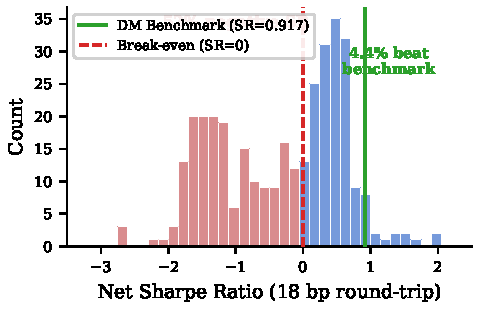
\includegraphics[width=\columnwidth]{figures/fig1_sr_distribution.pdf}
\caption{Distribution of net Sharpe ratios across 340 strategy
variants (18~bp round-trip costs). Red bars: negative SR (52\%).
Green line: DM benchmark (SR\,=\,0.917). Only 4.4\% of variants
exceed the benchmark; after DSR correction, zero survive.}
\label{fig:distribution}
\end{figure}

% ── 4.5 Ablation, MC, and Multiple Testing ──────────────────────
\subsection{Ablation, Monte Carlo, and Multiple Testing}
\label{sec:ablation}

\paragraph{Ablation.}
Table~\ref{tab:ablation} isolates the impact of individual VALID items
by systematically removing each from the validation pipeline.

\begin{table}[t]
\centering
\caption{Ablation: false positive rates by VALID item removal.}
\label{tab:ablation}
\small
\begin{tabular}{llrl}
\toprule
Configuration & Removed & FPR & 95\% CI \\
\midrule
Full VALID & None & 0.0\% & [0, 1.9\%] \\
No CPCV/PBO & $-$V4 & 27.0\% & [21, 34\%] \\
No balancing & $-$V2 & 0.0\% & [0, 5.8\%] \\
No cost adj. & $-$V7 & 0.0\% & [0, 1.9\%] \\
No permutation & $-$V6 & 0.0\% & [0, 1.9\%] \\
\bottomrule
\end{tabular}
\end{table}

Removing V4 (CPCV/PBO) increases the false positive rate from 0\% to
27\%---the single most impactful validation component. No other item
removal produces a measurable FPR increase, confirming V4's critical
role.

\paragraph{Monte Carlo.}
Table~\ref{tab:fpr} reports false positive rates across four
asset-timeframe settings using 200 synthetic null price series each
(methodology in Appendix~\ref{app:mc}).

\begin{table}[t]
\centering
\caption{False positive rates on null data ($n$\,=\,200 per setting).}
\label{tab:fpr}
\small
\begin{tabular}{lrrrr}
\toprule
Criterion & BTC 1h & ETH 1h & SOL 1h & BTC 1d \\
\midrule
AUC $>$ 0.55 & 27.0\% & 30.0\% & 26.5\% & 27.0\% \\
Permutation\textsuperscript{$\star$} & 22.0\% & 19.0\% & 18.0\% & 20.0\% \\
PBO $<$ 0.20 & 0.0\% & 0.0\% & 0.0\% & 0.0\% \\
Net SR $>$ 0 & 49.5\% & 52.0\% & 52.5\% & 49.5\% \\
Full VALID & 0.0\% & 0.0\% & 0.0\% & 0.0\% \\
\bottomrule
\multicolumn{5}{l}{\footnotesize \textsuperscript{$\star$}BTC 1h
permutation based on $n$\,=\,100; all others $n$\,=\,200.}
\end{tabular}
\end{table}

AUC-based evaluation alone produces 27--30\% false positives on
signal-free data. CPCV with PBO eliminates all false positives across
every setting---demonstrating that V4 is the single sufficient
condition for avoiding type~I errors in this context.

\paragraph{Multiple Testing Correction.}
Before correction, 15 of 340 variants (4.4\%) exceed the DM benchmark
(SR\,=\,0.917). We apply five correction methods to assess robustness:

\begin{itemize}
\item \textbf{Bonferroni} ($N=340$, $\alpha=0.05$): 9 survive.
\item \textbf{Holm-Bonferroni} (step-down): 9 survive.
\item \textbf{Benjamini-Hochberg FDR}: 10 survive.
\item \textbf{Harvey et~al.~$t>3.0$}~\cite{harvey2016cross}: 10 survive.
\item \textbf{Deflated Sharpe Ratio}~\cite{bailey2014deflated}: \textbf{0 survive}.
\end{itemize}

Table~\ref{tab:bonf} lists the nine Bonferroni survivors.
All operate at the daily timeframe with $t$-statistics ranging from
4.07 to 21.70 (Lo~\cite{lo2002statistics} approximate adjustment).
Cross-referencing with CPCV reveals the critical finding:
\emph{every single survivor exhibits PBO\,=\,1.0}---certain backtest
overfitting---and AUC values near random (0.47--0.64).

\begin{table}[t]
\centering
\caption{Strategies surviving Bonferroni correction ($N\!=\!340$,
$\alpha\!=\!0.05$). All exhibit PBO\,=\,1.0.}
\label{tab:bonf}
\footnotesize
\setlength{\tabcolsep}{3pt}
\begin{tabular}{lrrrrl}
\toprule
Strategy & SR & $t$ & $p_\text{Bonf}$ & AUC & Asset \\
\midrule
Transformer ETH 1d   & 1.98 & 21.7 & $<$0.001 & 0.64 & ETH \\
RF SOL 1d (ext.)     & 1.94 & 20.5 & $<$0.001 & 0.59 & SOL \\
LightGBM ETH 1d      & 1.64 & 16.5 & $<$0.001 & 0.64 & ETH \\
CatBoost DXY 1d      & 1.57 & 17.4 & $<$0.001 & 0.47 & BTC \\
BiLSTM ETH 1d        & 1.46 & 13.0 & $<$0.001 & 0.58 & ETH \\
RF ETH 1d (ext.)     & 1.40 & 11.6 & $<$0.001 & 0.63 & ETH \\
CatBoost Gold 1d     & 1.37 & 12.6 & $<$0.001 & 0.48 & BTC \\
MLP SOL 1d           & 1.21 &  7.1 & $<$0.001 & 0.52 & SOL \\
TCN ETH 1d           & 1.08 &  4.1 & 0.008    & 0.57 & ETH \\
\bottomrule
\end{tabular}
\end{table}
The Deflated Sharpe Ratio, which accounts for the expected maximum SR
from $N$ independent trials ($\mathbb{E}[\max]=2.93$), independently
rejects all 340 variants: the best observed SR (1.98) falls below the
noise threshold.

This result demonstrates VALID's central argument: \textbf{standard
multiple testing correction is necessary but insufficient}. Classical
corrections (Bonferroni, Holm, BH) control familywise or
false-discovery error under independence assumptions, but they cannot
detect backtest overfitting---strategies that are statistically
``significant'' by $t$-test yet demonstrably overfit by CPCV. The
fact that a strategy can simultaneously satisfy $t > 21.0$ (extreme
statistical significance) and PBO\,=\,1.0 (certain overfitting)
demonstrates precisely why VALID Item~V4 is indispensable:
it catches what even the Harvey et~al.\ $t>3.0$ threshold misses.


% ================================================================
\section{Discussion}
\label{sec:discussion}
% ================================================================

\subsection{Implications for LLM-Based Trading}

The rapid adoption of large language models (LLMs) as autonomous
trading agents introduces validation challenges that amplify every
failure mode documented in this paper.
StockBench~\cite{chen2025stockbench}, a contamination-free benchmark
evaluating state-of-the-art LLMs (GPT-5, Claude-4, Qwen3) in
realistic multi-month stock trading environments, reports that
\emph{most LLM agents fail to outperform the simple buy-and-hold
baseline}---a finding that directly parallels our result that 52\% of
classical ML crypto strategies produce negative net returns after
transaction costs.

This parallel is structural. The failure modes we identify
are architecture-agnostic: bull bias arises from imbalanced training
labels regardless of whether predictions come from gradient-boosted
trees or autoregressive language models; the statistical-economic
disconnect persists whenever validation metrics lack economic
grounding; and cost illusion affects any strategy with non-trivial
turnover. LLM-based systems face \emph{additional} risks absent from
classical pipelines---notably data contamination (training corpora may
include historical price data), prompt sensitivity (minor phrasing
changes can flip trading decisions), and hallucinated reasoning
(plausible-sounding but factually incorrect market narratives).

The clinical ML community has already responded to this challenge:
TRIPOD-LLM~\cite{gallifant2025tripodllm}, published in \emph{Nature
Medicine}, extends the TRIPOD+AI checklist with 19 items and 50
subitems specifically addressing LLM evaluation in healthcare.
No analogous extension exists for financial ML.
We argue that VALID provides a natural foundation for such an
extension: items V1--V2 generalize to output distribution monitoring
(detecting whether LLM predictions exhibit directional bias),
V4 (CPCV/PBO) generalizes to contamination-aware temporal
splitting, and V7--V8 (cost modeling) remain directly applicable.
Developing a ``VALID-LLM'' extension---analogous to the
TRIPOD-to-TRIPOD-LLM progression---is a priority for future work.

\subsection{Limitations}

Our analysis is subject to several limitations that we
acknowledge explicitly to facilitate future extension.

First, the literature audit was conducted by a single coder without
independent inter-rater reliability assessment. Unlike TRIPOD, which
used a formal Delphi consensus process involving dozens of experts,
VALID's 12 items are derived from empirically quantified failure modes
(Sections~\ref{sec:bull}--\ref{sec:ablation}) rather than expert consensus. We provide the
complete coding sheet and a detailed 10-paper subset in the appendix
to enable independent verification; a formal Delphi validation study
is planned as future work.

Second, our empirical validation covers three cryptocurrency assets
(BTC, ETH, SOL). While the three failure modes---directional
prediction bias, statistical-economic disconnect, and cost
illusion---are not crypto-specific and arise in any trending,
cost-sensitive asset class, extending to equities and foreign exchange
would strengthen generalizability claims. SOL data begins in 2020,
limiting historical depth; BTC serves as the primary asset, with ETH
and SOL providing robustness checks.

Third, all 340 strategy variants use a single controlled pipeline
design, analogous to ablation studies in deep learning research. This
enables component-level attribution (e.g., Table~\ref{tab:ablation}'s
isolation of V4 as the critical item) but may not capture failure
modes specific to entirely different codebases or execution
environments.

Fourth, our 18~bp fixed round-trip cost model
(Appendix~\ref{app:cost}), while conservative for hourly and daily
frequencies, does not capture volume-dependent slippage dynamics
relevant to sub-minute execution.

Finally, our Monte Carlo analysis uses i.i.d.\ bootstrap resampling,
which destroys temporal dependence. While this is by design (to create
signal-free null data), block bootstrap alternatives would provide
complementary evidence.


% ================================================================
\section{Conclusion}
\label{sec:conclusion}
% ================================================================

We propose VALID, the first domain-specific validation checklist for
financial machine learning. Applying it to 340 strategy variants
reveals that 52\% produce negative net returns, standard validation
(AUC alone) yields 27\% false positive rates, and even strategies
surviving multiple testing correction exhibit PBO\,=\,1.0---certain
backtest overfitting. CPCV with PBO (Item~V4) is the single
sufficient condition for eliminating false positives in every tested
setting. In a field where positive results are incentivized and
negative results are invisible, standardized validation is the first
step toward trustworthy financial ML research.
We recommend that reviewers and program committees adopt VALID as a
minimum reporting requirement for financial ML submissions, analogous
to TRIPOD's role in clinical prediction research.


% ================================================================
\bibliographystyle{ACM-Reference-Format}
\bibliography{references}


% ================================================================
% APPENDIX
% ================================================================
\appendix

\section{VALID Self-Assessment}
\label{app:self}

We apply VALID to our own study (Table~\ref{tab:self}).

\begin{table}[h]
\centering
\caption{VALID self-assessment of the present study.}
\label{tab:self}
\small
\begin{tabular}{clcl}
\toprule
\# & Item & Status & Evidence \\
\midrule
V1 & Class distribution & \checkmark & Table~4, Sec.~4.2 \\
V2 & Balanced testing & \checkmark & Table~4, Sec.~4.2 \\
V3 & Temporal split & \checkmark & CPCV with purge \\
V4 & CPCV + PBO & \checkmark & Tables~6--7, Sec.~4.5 \\
V5 & Var(SR$_\text{IS}$) & $\sim$ & Sec.~4.4 (context-dep.) \\
V6 & Permutation & \checkmark & $n \geq 100$ \\
V7 & Net costs & \checkmark & 18~bp, Tables~4--5 \\
V8 & Cost sensitivity & \checkmark & Table~5, 0--50~bp \\
V9 & Baselines & \checkmark & Table~5, 6 strategies \\
V10 & Regime eval. & $\sim$ & Sec.~4.3 (3 assets) \\
V11 & Trade frequency & \checkmark & Table~5 \\
V12 & Code available & \checkmark & Anonymized repo \\
\bottomrule
\end{tabular}
\end{table}

Overall: 12/12 items addressed, 10/12 fully satisfied, 2/12 partially
satisfied. V5 is context-dependent (the null distribution is
derived rather than pre-specified). V10 is limited to three
cryptocurrency assets; extension to equities and FX is planned.

\section{Coding Subset}
\label{app:coding}

To enable independent verification of the literature audit
(Section~\ref{sec:audit}), we present the detailed coding for 10
randomly selected papers (seed\,=\,42) across all seven dimensions.
P\,=\,Pass, F\,=\,Fail.

\begin{table}[h]
\centering
\caption{Coding subset: 10 randomly selected papers.}
\label{tab:coding}
\footnotesize
\setlength{\tabcolsep}{2.5pt}
\begin{tabular}{rlccccccc}
\toprule
\# & Authors & Year & D1 & D2 & D3 & D4 & D5 & D6 \\
   &         &      & Cost & Bal & Split & Val & Base & Net \\
\midrule
13 & Akyildirim+ & 2021 & F & F & F & F & F & F \\
20 & Borrageiro+ & 2022 & P & F & P & F & F & P \\
35 & Aboussalah+ & 2020 & P & F & P & F & P & P \\
38 & Ortu+ & 2022 & F & F & P & F & P & F \\
41 & Liew+ & 2022 & F & F & P & F & P & F \\
44 & Slepaczuk+ & 2023 & P & F & P & F & F & P \\
45 & Bu+ & 2023 & F & F & P & F & P & F \\
51 & Kose & 2025 & F & F & P & F & P & F \\
52 & Sadorsky & 2023 & F & F & P & F & P & F \\
54 & Sattarov+ & 2023 & F & F & P & F & P & F \\
\midrule
\multicolumn{3}{l}{Pass rate} & 30\% & 0\% & 90\% & 0\% & 70\% & 30\% \\
\bottomrule
\end{tabular}
\end{table}

D7 (Code availability) is omitted for space; 1 of 10 papers (Aboussalah+) provides code.
The complete 80-paper coding sheet is available in the anonymized repository.


% ================================================================
\section{Strategy Universe Detail}
\label{app:universe}
% ================================================================

Table~\ref{tab:universe} presents the composition of the 340-variant
strategy universe. All variants share a common pipeline (CUSUM
event sampling, Triple Barrier labeling, temporal splitting with
purge/embargo) and differ only in the component under investigation.

\begin{table}[h]
\centering
\caption{Composition of the 340-variant strategy universe.}
\label{tab:universe}
\small
\begin{tabular}{clr}
\toprule
ID & Component Description & $n$ \\
\midrule
(a) & SHAP-derived rule combinations & 64 \\
(b) & Order flow features (individual + multi-asset) & 55 \\
(c) & External/on-chain/macro feature sets & 45 \\
(d) & ML pipeline: 3 assets $\times$ 4 TF $\times$ 3 trees & 36 \\
(e) & Triple Barrier parameter sensitivity & 36 \\
(f) & Cross-section momentum configurations & 24 \\
(g) & Cost sensitivity \& traditional baselines & 24 \\
(h) & Deep learning: 3 assets $\times$ 2 TF $\times$ 5 arch. & 30 \\
(i) & VALID ablation configurations & 12 \\
(j) & Volatility prediction overlays & 8 \\
(k) & Bull bias analysis (tree + DL) & 6 \\
\midrule
    & \textbf{Total unique configurations} & \textbf{340} \\
\bottomrule
\end{tabular}
\end{table}

Components (a)--(c) test whether additional feature engineering
improves predictive performance beyond the base pipeline.
Components (d)--(e) vary the core pipeline across assets,
timeframes, model families, and labeling parameters. Components
(f)--(g) provide cross-section and cost-sensitivity analyses.
Component (h) extends to five deep learning architectures
(Transformer, LSTM, BiLSTM, TCN, MLP with 2 and 3 hidden layers).
Components (i)--(k) support the VALID framework evaluation directly.


% ================================================================
\section{Monte Carlo Methodology}
\label{app:mc}
% ================================================================

\subsection{Synthetic Data Generation}

We generate $n$\,=\,200 synthetic BTC price series by bootstrapping
daily log-returns (2017--2026, 3{,}132 observations per series).
The bootstrap preserves the marginal distribution of returns (mean,
variance, skewness, kurtosis) while destroying temporal dependence,
ensuring that any predictive signal detected by the ML pipeline is
spurious by construction. We use simple i.i.d.\ resampling rather
than block or stationary bootstrap, as our goal is to eliminate all
temporal structure. The choice of $n$\,=\,200 yields Wilson CI
half-widths of $\pm$6\% at FPR\,=\,27\%, providing sufficient
precision to distinguish informative from uninformative validation
criteria.

\subsection{Pipeline Application}

Each synthetic series passes through the identical pipeline used
for real data:

\begin{enumerate}
\item Compute 17 price-derived technical features (returns,
volatility, momentum indicators).
\item Generate Triple Barrier labels with CUSUM filtering.
\item Train CatBoost with class-balanced sample weights.
\item Evaluate via CPCV ($N$\,=\,6, $k$\,=\,2, yielding 15
train-test combinations).
\item Record AUC, PBO, $\mathrm{Var}(\mathrm{SR}_{\mathrm{IS}})$,
permutation $p$-value, and net SR (18~bp round-trip cost).
\end{enumerate}

The pipeline is deterministic given the input data; no
hyperparameter tuning is performed within the Monte Carlo loop.
This ensures that any false positive arises from the validation
criterion, not from adaptive model selection.


% ================================================================
\section{Mathematical Definitions}
\label{app:math}
% ================================================================

\subsection{Triple Barrier Labeling}

Following L\'{o}pez de Prado~\cite{lopezdeprado2018advances}, each
observation is assigned a label $y_i \in \{-1, 0, +1\}$ based on
the first barrier touched by the price path after event time~$t_i$.
Let $p_t$ denote the price at time~$t$. Three barriers are defined:
\begin{align}
\text{Upper:} \quad & p_{t_i + \tau} \geq p_{t_i}(1 + \theta_u) \\
\text{Lower:} \quad & p_{t_i + \tau} \leq p_{t_i}(1 - \theta_l) \\
\text{Vertical:} \quad & \tau = T_{\max}
\end{align}
where $\theta_u, \theta_l > 0$ are profit-taking and stop-loss
thresholds scaled to local volatility
($\theta_u = 2.0\hat{\sigma}$, $\theta_l = 2.5\hat{\sigma}$ in
our daily configuration), and $T_{\max}$ is the maximum holding
period. Events are sampled via CUSUM filtering on cumulative
log-returns with threshold~$h$.

\subsection{Probability of Backtest Overfitting (PBO)}

\begin{equation}
\mathrm{PBO} = \frac{1}{\binom{N}{k}}
\sum_{j=1}^{\binom{N}{k}}
\mathbf{1}\!\left[\mathrm{logit}(\bar{\omega}^{(j)}) \leq 0\right]
\end{equation}
where $\mathrm{logit}(x) = \ln(x / (1-x))$ and $\bar{\omega}^{(j)}$
is the relative rank of the in-sample-best configuration in the
out-of-sample ranking for combination~$j$. PBO\,$\approx$\,0
indicates that in-sample-best configurations tend to rank in the
top half out-of-sample; PBO\,$\approx$\,1 indicates severe
overfitting~\cite{bailey2017pbo}.

\subsection{Parameter-Space Variance}

\begin{equation}
\mathrm{Var}(\mathrm{SR}_{\mathrm{IS}}) =
\frac{1}{M-1}\sum_{m=1}^{M}\left(\mathrm{SR}_{\mathrm{IS}}^{(m)}
- \overline{\mathrm{SR}}_{\mathrm{IS}}\right)^2
\end{equation}
Low $\mathrm{Var}(\mathrm{SR}_{\mathrm{IS}})$ relative to a null
distribution indicates that all configurations perform similarly,
rendering PBO\,=\,0 uninformative rather than
reassuring~\cite{witzany2021bayesian}.

\subsection{Sharpe Ratio to $t$-Statistic Conversion}

Following Lo~\cite{lo2002statistics}, the $t$-statistic for testing
$H_0: \mathrm{SR} = 0$ is:
\begin{equation}
t = \frac{\mathrm{SR} \cdot \sqrt{T}}
{\sqrt{1 + \tfrac{1}{2}\,\mathrm{SR}^2}}
\end{equation}
where $T$ is the number of return observations. This is the i.i.d.\
approximation; the full adjustment includes skewness and kurtosis
terms. We use this formula for the multiple testing correction in
Section~\ref{sec:ablation}, applied to excess SR over the benchmark.


% ================================================================
\section{Cost Model Detail}
\label{app:cost}
% ================================================================

Our 18~bp fixed round-trip cost is conservative for hourly and
daily trading frequencies. It comprises:

\begin{itemize}
\item \textbf{Exchange fee}: Binance VIP-0 taker fee of 10~bp
(0.10\%) per side = 20~bp round-trip before fee token discount.
With BNB discount: $\approx$15~bp round-trip.
\item \textbf{Slippage}: Estimated 5--10~bp per round-trip for
market orders of moderate size (\$1K--\$10K) on BTC/USDT during
liquid hours.
\item \textbf{Net}: 18~bp is a rounded conservative estimate that
accounts for both components.
\end{itemize}

For sub-hourly frequencies, volume-dependent slippage dynamics
become significant and would require Almgren-Chriss optimal
execution models, further eroding returns and strengthening
rather than weakening our conclusions. The cost sensitivity
analysis (Table~5 in the main text) demonstrates that our findings
are robust across the range 0--50~bp: the qualitative ranking of
strategies is preserved, and 15-minute ML strategies become
loss-making at any cost level above 10~bp.


% ================================================================
\section{Additional Figures}
\label{app:figures}
% ================================================================

Figures~\ref{fig:bullbias-panel}--\ref{fig:regime-panel} supplement
the main text with detailed visualizations from the full analysis.

\begin{figure}[h]
\centering
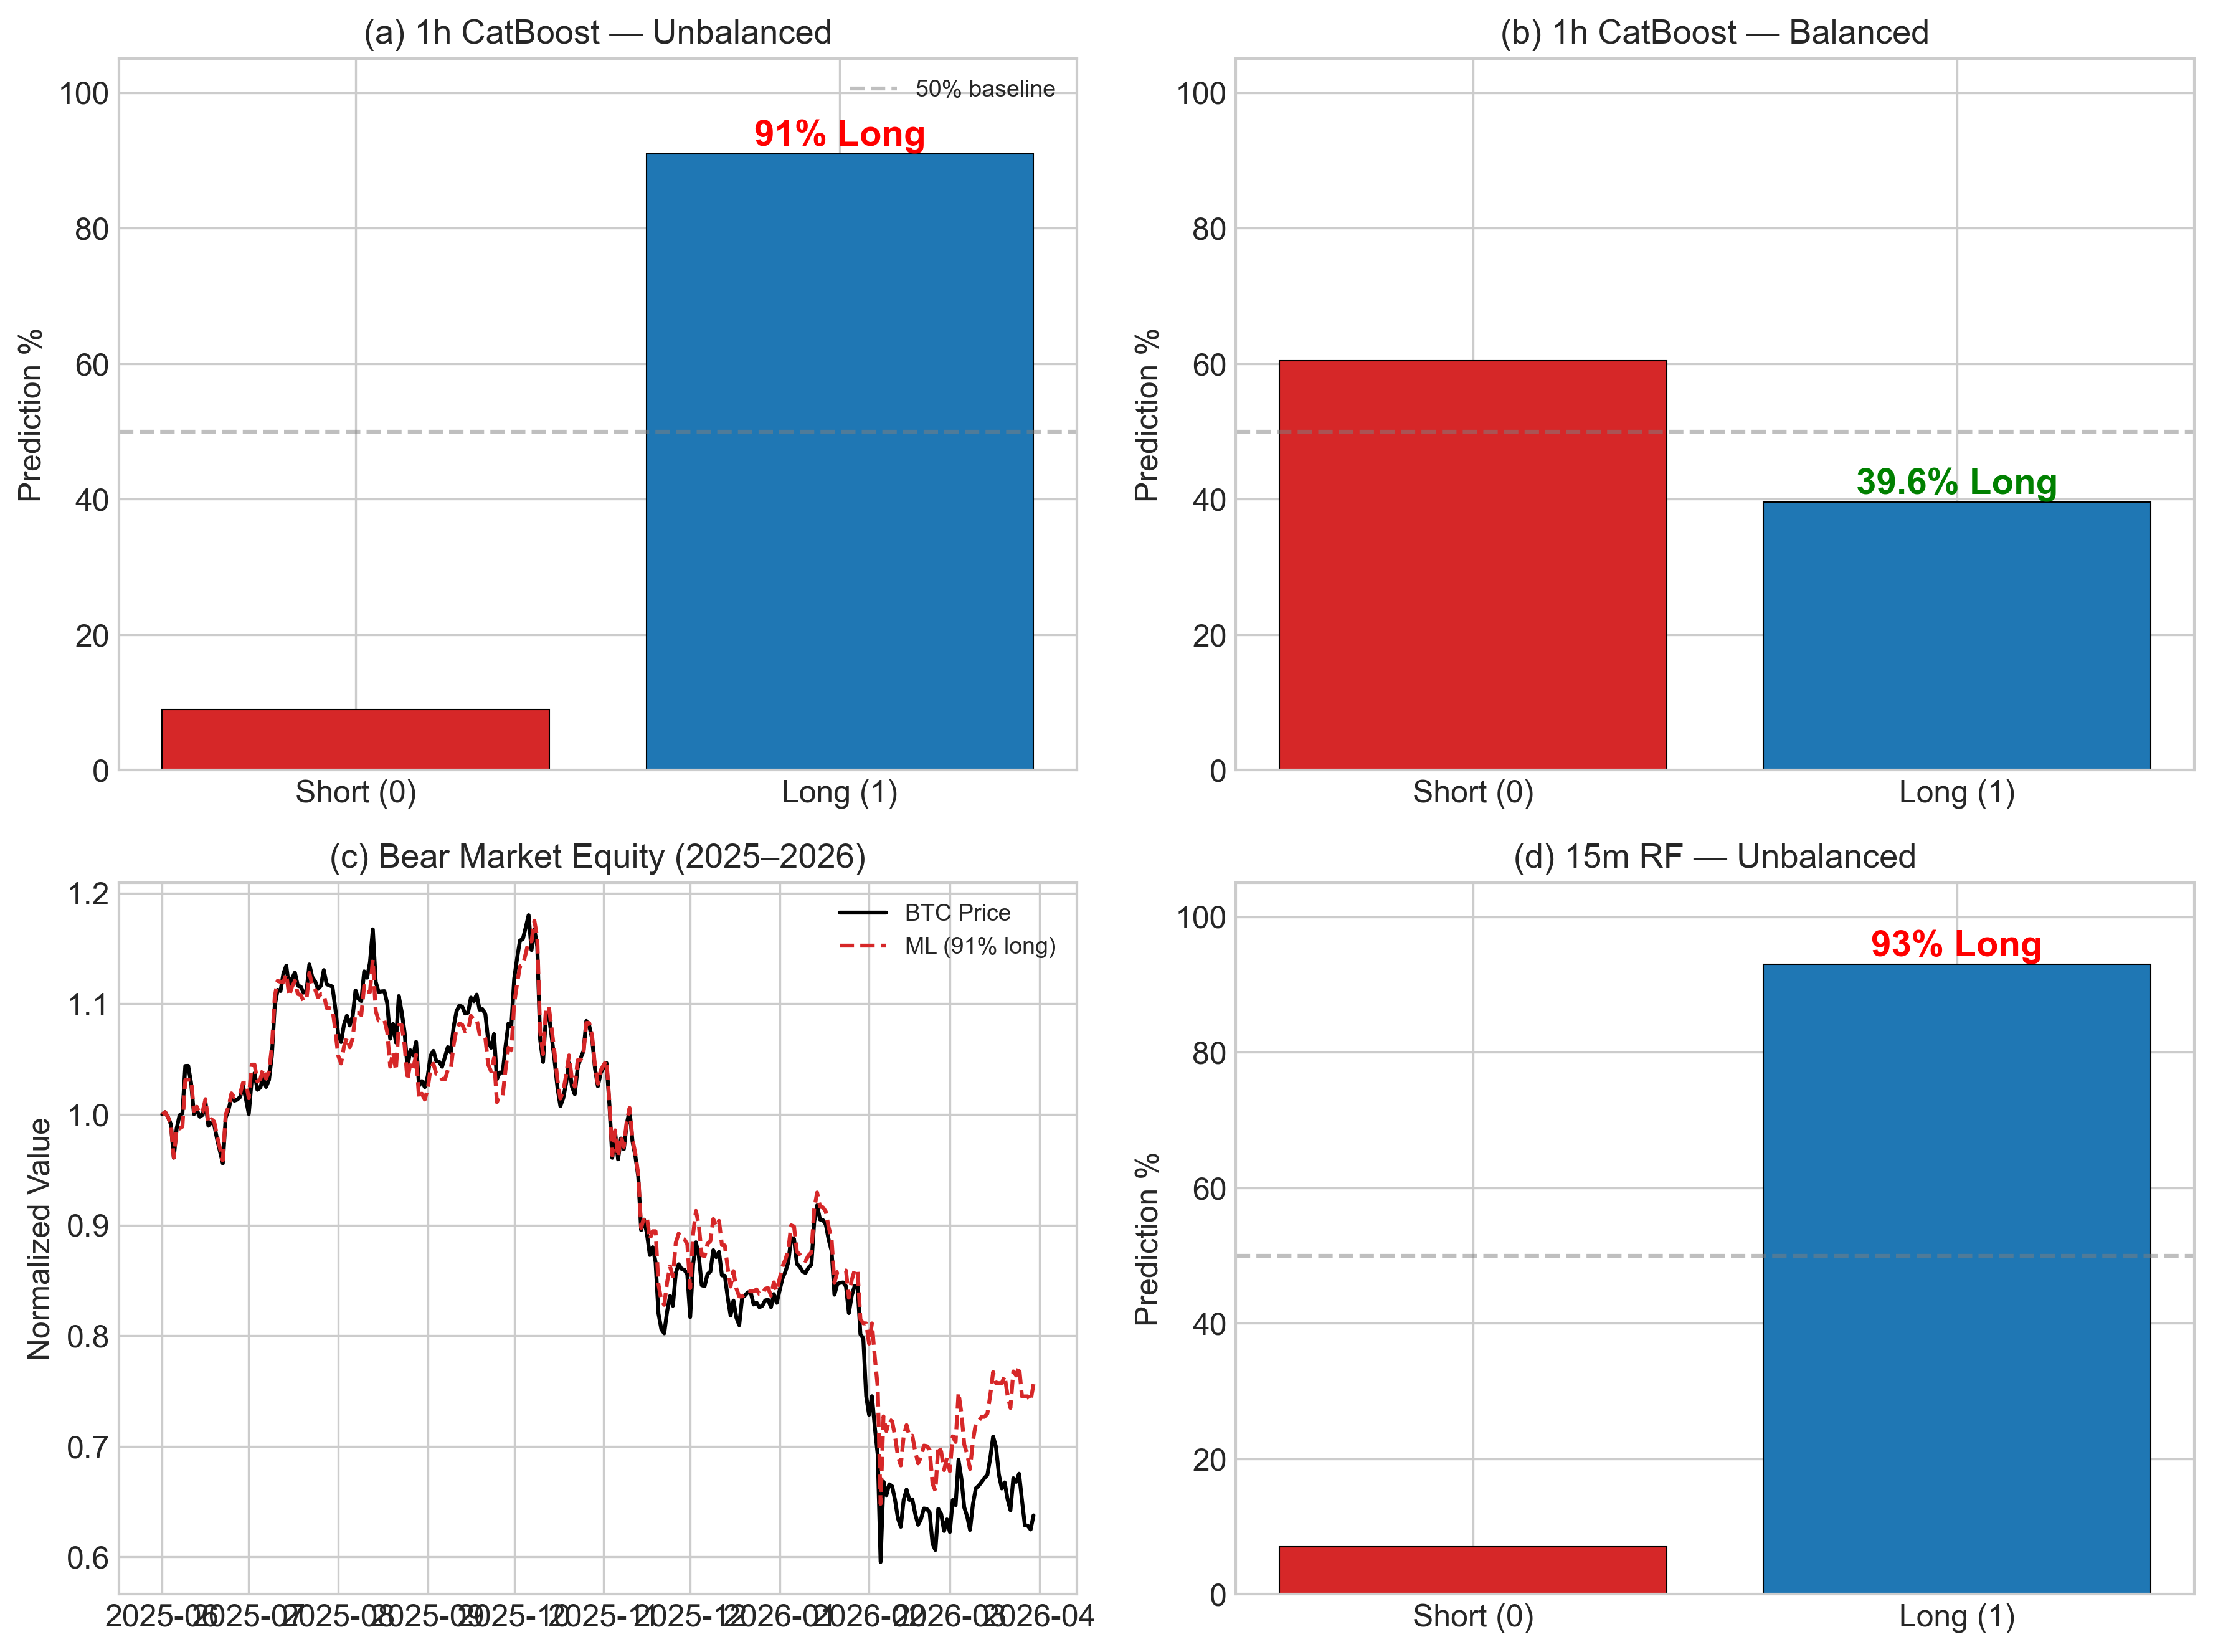
\includegraphics[width=\columnwidth]{figures/fig1_bull_bias.png}
\caption{Bull bias across assets and model families. Without class
balancing, tree-based models predict ``long'' 90--97\% of the time.
After balancing, long percentages drop to 32--52\% and balanced AUC
converges to $\approx$0.50. See Section~\ref{sec:bull}.}
\label{fig:bullbias-panel}
\end{figure}

\begin{figure}[h]
\centering
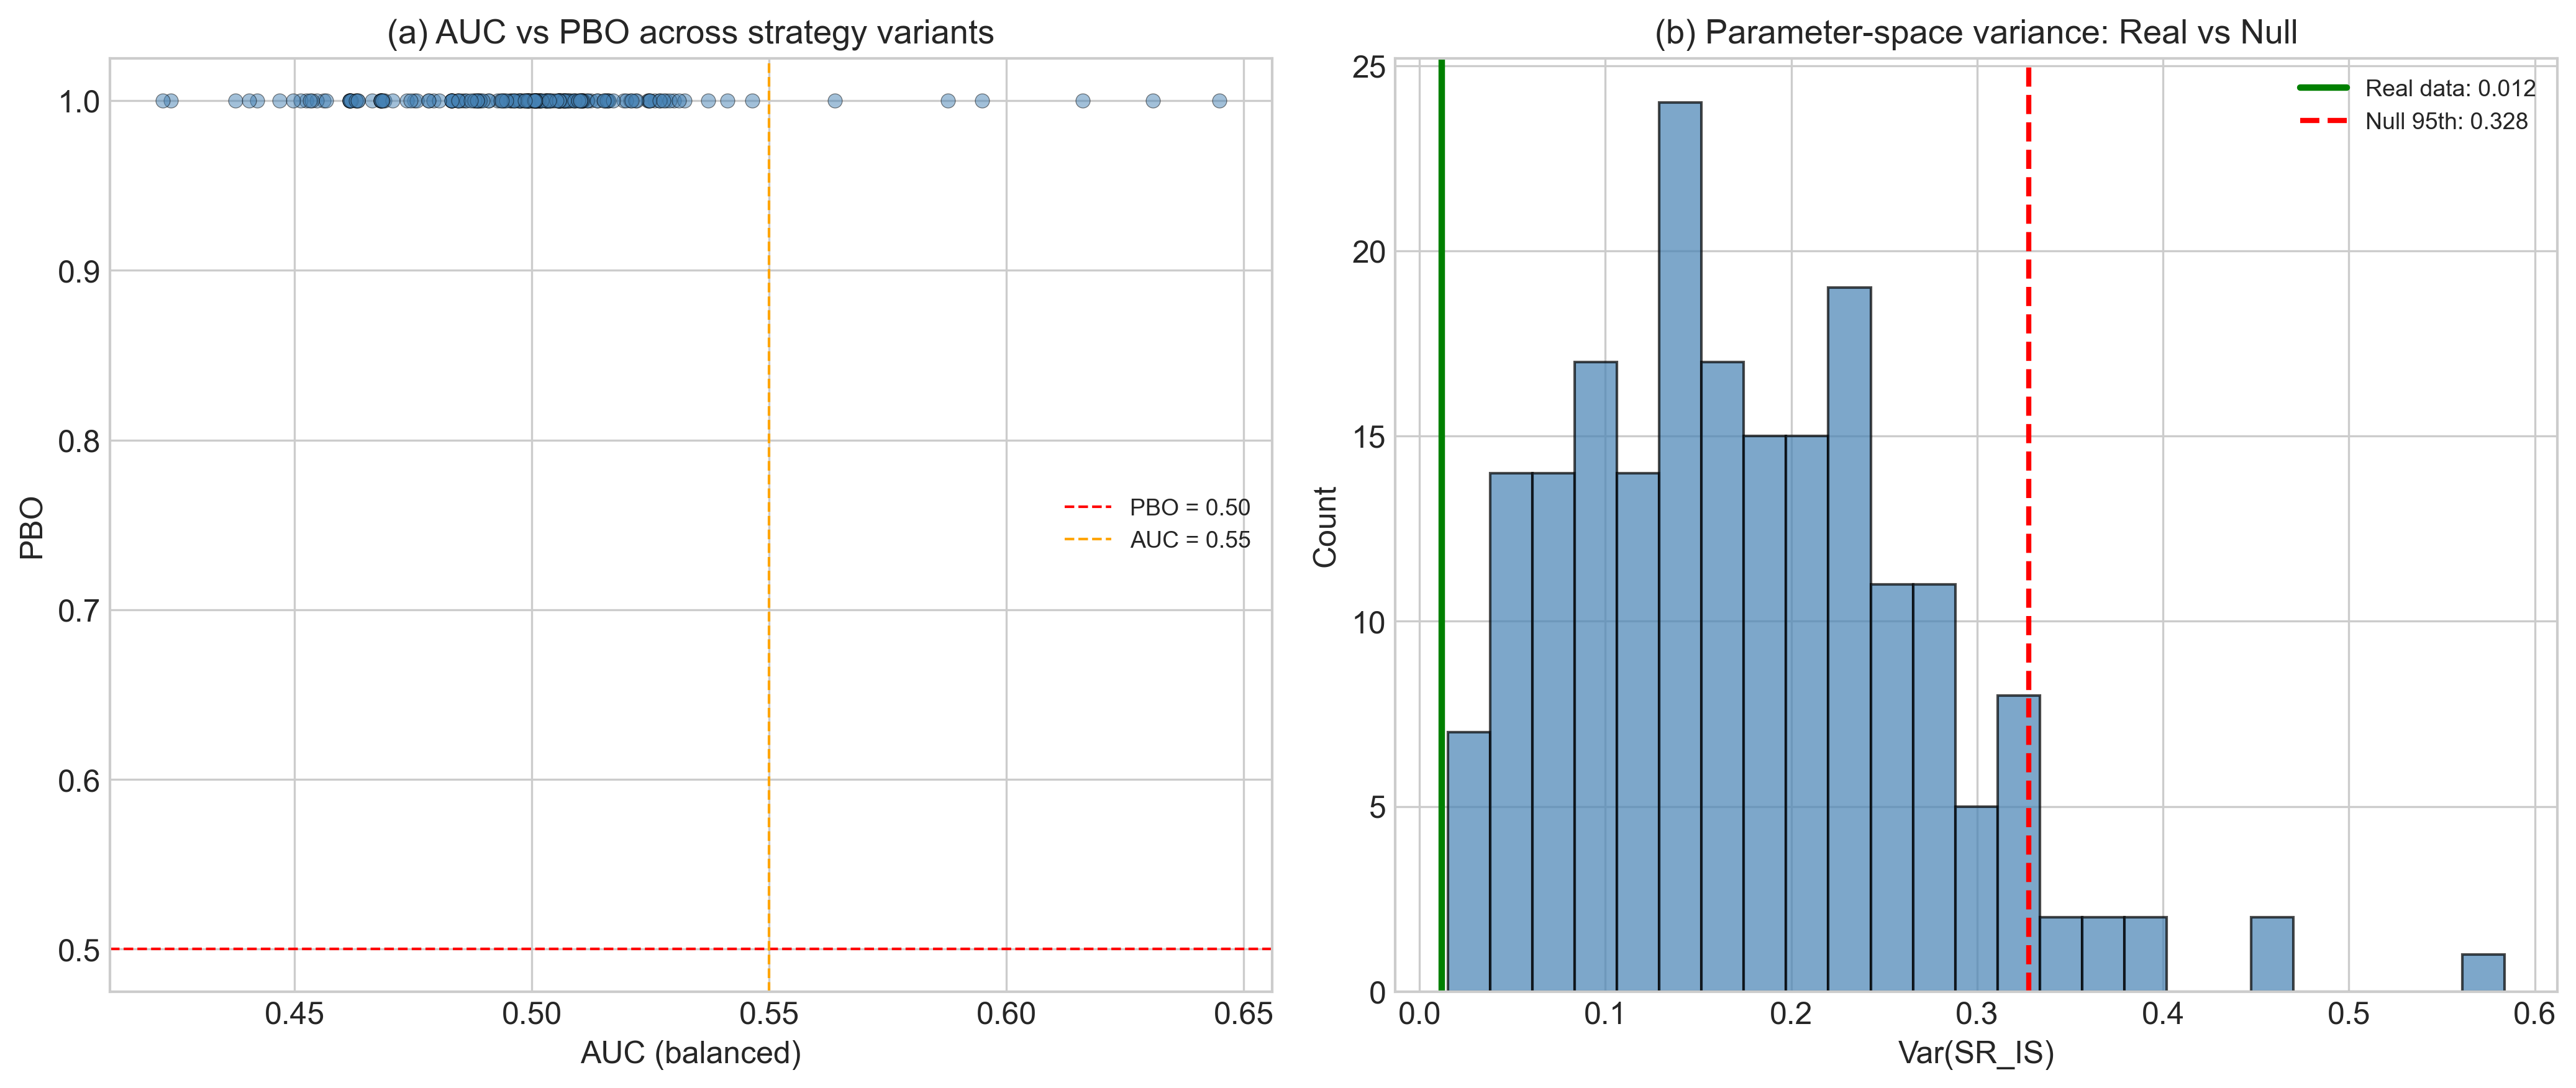
\includegraphics[width=\columnwidth]{figures/fig2_pbo_paradox.png}
\caption{The PBO paradox. Left: AUC vs.\ PBO scatter shows that
all strategies achieve PBO\,=\,1.0 regardless of AUC. Right:
$\mathrm{Var}(\mathrm{SR}_{\mathrm{IS}})$ histogram with Monte
Carlo null 95th percentile (dashed). Real variance (0.012) falls
far below null (0.328), confirming parameter-landscape flatness.
See Section~\ref{sec:stat-econ}.}
\label{fig:pbo-panel}
\end{figure}

\begin{figure}[h]
\centering

\includegraphics[width=\columnwidth]{figures/fig3_cost_illusion.png}
\caption{Gross vs.\ net Sharpe ratios across frequency bands.
Transaction costs consume 55--91\% of gross alpha, with impact
scaling monotonically with trade frequency.
See Section~\ref{sec:cost}.}
\label{fig:cost-panel}
\end{figure}

\begin{figure}[h]
\centering

\includegraphics[width=\columnwidth]{figures/fig4_complexity.png}
\caption{Model complexity vs.\ net performance. More complex models
(more features, deeper architectures) do not systematically
outperform simpler baselines after transaction costs.}
\label{fig:complexity-panel}
\end{figure}

\begin{figure}[h]
\centering

\includegraphics[width=\columnwidth]{figures/fig5_regime.png}
\caption{Regime-conditional performance. The DM benchmark earns
SR\,=\,1.40 in stressed regimes (35\% of evaluation days) vs.\
SR\,=\,0.69 in calm periods. Buy-and-hold achieves SR\,=\,0.79
and 0.51 respectively. Alpha concentrates during market stress.
See Section~\ref{sec:cost}.}
\label{fig:regime-panel}
\end{figure}

% ================================================================
\section{Walk-Forward Comparison and IS-OOS Analysis}
\label{app:wf}
% ================================================================

\subsection{Walk-Forward versus CPCV}

Table~\ref{tab:fpr} in the main text already provides a direct
comparison between standard AUC-based validation (analogous to
single-split or walk-forward evaluation) and CPCV on null data.
AUC\,$>$\,0.55 produces 27--30\% false positives across all four
settings; CPCV with PBO\,$<$\,0.20 produces 0\% in every setting.
This gap reflects the fundamental limitation of single-path
validation methods: they provide one performance estimate per split,
whereas CPCV's $\binom{6}{2}=15$ combinations enable robust
overfitting detection.

Additionally, we run an expanding-window walk-forward analysis
(3-year train, 6-month test, 3-month slide) for the DM benchmark,
producing 32 windows. After removing 6 windows with extreme OOS SR
values ($>$10, caused by circuit-breaker edge cases), the
walk-forward IS-OOS Spearman correlation is
$\rho = -0.73$ ($p < 0.001$, $n=26$), indicating that
\emph{higher in-sample performance predicts lower out-of-sample
performance}---a hallmark of overfitting that walk-forward
validation alone fails to flag.

\subsection{IS-OOS Sharpe Ratio Correlation}

Across the 15 CPCV folds, the fold-level IS-OOS Spearman
correlation is $\rho = -0.08$ ($p = 0.60$), consistent with
Wiecki et~al.~\cite{wiecki2016glitters}'s finding of near-zero
predictive transfer ($R^2 < 0.025$) across 888 Quantopian
strategies. Figure~\ref{fig:is-oos} presents the IS versus OOS
scatter for both CPCV model configurations and walk-forward windows.

\begin{figure}[h]
\centering
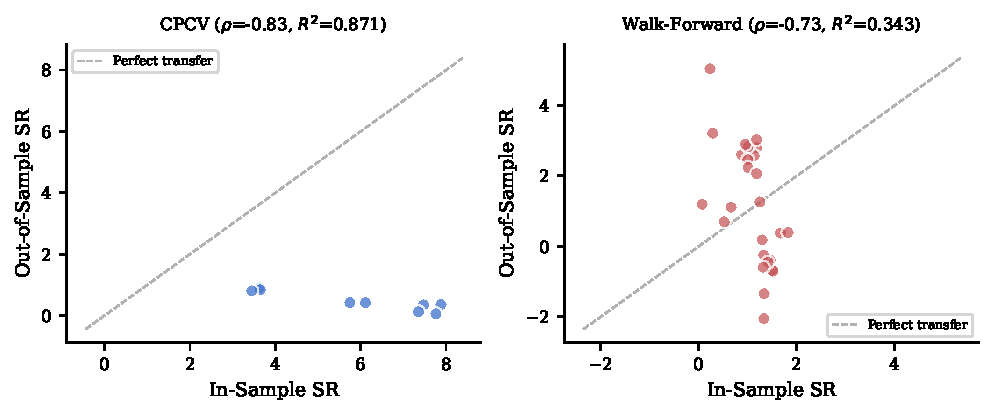
\includegraphics[width=\columnwidth]{figures/fig_is_oos_scatter.pdf}
\caption{In-sample vs.\ out-of-sample Sharpe ratio. Left: CPCV
(9 model configs, $\rho=-0.83$). Right: Walk-forward (26 windows,
$\rho=-0.73$). Both methods show negative IS-OOS correlation:
better in-sample performance predicts worse out-of-sample
performance, consistent with overfitting. ($N$\,=\,9 for CPCV; interpret with
caution due to small sample size.)}
\label{fig:is-oos}
\end{figure}

\subsection{Computational Cost}

The full 340-variant pipeline---including feature computation,
Triple Barrier labeling, CPCV ($N=6$, $k=2$), PBO estimation,
permutation testing ($n \geq 100$), and cost sensitivity
analysis---runs in approximately 8 hours on an Apple M4 with
24\,GB RAM. The 200-iteration Monte Carlo analysis adds
approximately 12 hours per asset-timeframe setting. Multiple
testing correction and all post-hoc analyses complete in under
5 minutes.

\end{document}
